\documentclass[10pt, a4paper, conference, compsocconf]{IEEEtran}
% Some Computer Society conferences also require the compsoc mode option,
% but others use the standard conference format.
%
% If IEEEtran.cls has not been installed into the LaTeX system files,
% manually specify the path to it like:
% \documentclass[conference]{../sty/IEEEtran}

% *** CITATION PACKAGES ***
%
\usepackage{url}
\usepackage{cite}
% cite.sty was written by Donald Arseneau
% V1.6 and later of IEEEtran pre-defines the format of the cite.sty package
% \cite{} output to follow that of IEEE. Loading the cite package will
% result in citation numbers being automatically sorted and properly
% "compressed/ranged". e.g., [1], [9], [2], [7], [5], [6] without using
% cite.sty will become [1], [2], [5]--[7], [9] using cite.sty. cite.sty's
% \cite will automatically add leading space, if needed. Use cite.sty's
% noadjust option (cite.sty V3.8 and later) if you want to turn this off
% such as if a citation ever needs to be enclosed in parenthesis.
% cite.sty is already installed on most LaTeX systems. Be sure and use
% version 5.0 (2009-03-20) and later if using hyperref.sty.
% The latest version can be obtained at:
% http://www.ctan.org/tex-archive/macros/latex/contrib/cite/
% The documentation is contained in the cite.sty file itself.

\usepackage[pdftex]{graphicx}
% declare the path(s) where your graphic files are
% \graphicspath{{../pdf/}{../jpeg/}}
% and their extensions so you won't have to specify these with
% every instance of \includegraphics
% \DeclareGraphicsExtensions{.pdf,.jpeg,.png}

% *** SPECIALIZED LIST PACKAGES ***
%
%\usepackage{algorithmic}
% algorithmic.sty was written by Peter Williams and Rogerio Brito.
% This package provides an algorithmic environment fo describing algorithms.
% You can use the algorithmic environment in-text or within a figure
% environment to provide for a floating algorithm. Do NOT use the algorithm
% floating environment provided by algorithm.sty (by the same authors) or
% algorithm2e.sty (by Christophe Fiorio) as IEEE does not use dedicated
% algorithm float types and packages that provide these will not provide
% correct IEEE style captions. The latest version and documentation of
% algorithmic.sty can be obtained at:
% http://www.ctan.org/tex-archive/macros/latex/contrib/algorithms/
% There is also a support site at:
% http://algorithms.berlios.de/index.html
% Also of interest may be the (relatively newer and more customizable)
% algorithmicx.sty package by Szasz Janos:
% http://www.ctan.org/tex-archive/macros/latex/contrib/algorithmicx/



% *** Do not adjust lengths that control margins, column widths, etc. ***
% *** Do not use packages that alter fonts (such as pslatex).         ***
% There should be no need to do such things with IEEEtran.cls V1.6 and later.
% (Unless specifically asked to do so by the journal or conference you plan
% to submit to, of course. )
% correct bad hyphenation here
\hyphenation{op-tical net-works semi-conduc-tor}


\begin{document}


\title{Concurrent Zombie Swarm Simulation}

\author{\IEEEauthorblockN{Joseph Mitchard}
\IEEEauthorblockA{University of Kent\\ Email: jm710@kent.ac.uk}
\and
\IEEEauthorblockN{Jake Pearse}
\IEEEauthorblockA{University of Kent\\ Email: jp480@kent.ac.uk}
\and
\IEEEauthorblockN{Robert S.J. Hales}
\IEEEauthorblockA{University of Kent\\ Email: rsjh3@kent.ac.uk}}
% make the title area
\maketitle

% As a general rule, do not put math, special symbols or citations
% in the abstract
\begin{abstract}
% what the fuck is an abstract?
The abstract goes here.
\end{abstract}

\section{Introduction \label{intro}}
% what is the project?
% what have we done?
% why have we done it? maybe
% what is in the rest of the document
zsxfcghadgbadfgbadfghba

Throughout the document we will introduce the \verb+swarmer+ application, as well as the client we have built to visualise the simulation, explaining how we have implemented the integral parts of the application. We will also introduce the behaviour models that we have created in order to make the different entitiy types within the simulation behave the way they do.\\
\\
% team stuff
In order to realsie our goals for the project, we had to learn a lot of new things. So as to achieve this, we had to take a diciplined and systematic approach to familiarise ourselves with these new concepts and libraries. Responsibility for researching and learning these technologies had to be deligated amongst the team members, and then regular updates to other members on the findings. This allowed us to familiarise ourselves with the new concepts as a group, within a limited space of time.\\
\\
The majority of development was carried out as a group, using techniques that are part of the extreme programming practice, and a large amount of pair programming.\\
\\
\section{Background \label{background}}
% research into the area
Erlang is an open-source programming language developed by Ericsson Computer Science Laboratory; it was originally designed for telecoms systems, but over the years has become a general-use functional and concurrent language.\\
\\
Javascript is a dynamic general-use programming language that is mostly used for web development. It has a large number of well supported and documented librarys that cover a wide range of areas. We have chosen to use the D3\cite{d3} library because of it's built in ability to dynamically manipulate data. It is reasonably lightweight and very good at manipulating and manging large amounts of data.\\
\\
Before deciding to implement the simulation based around entities in the Erlang programming language, we needed to ensure that the idea was a feasible one. We have found two noteworthy implementations of a crowd swarming simulation, one in OccamPi by Fred Barnes\cite{occam_boids}, a professor the University of Kent, and a second written in Erlang by Jim Menard\cite{erlang_boids}.\\
\\
% boids
The behavioural model we have implemented is based on the Boids Algorithm \cite{boids}, created by Craig Reynolds in 1986. The model focuses on steering behaviours to lead to crowd flocking, and is heavily used in animation and game development. Our modified version of the algorithm is described in section \ref{behaviours}.\\
\\
\section{Aims \label{aims}}
% what we set out to achieve
Our goal was to create a plausible simulation of a dynamic environment containing zombie and human entities. We wanted zombies to exhibit flocking behaviour and to hunt down humans within the environment, turning them into zombies when they are caught. \\
\\
In order to make the system more believeable, we wanted to implement certain behaviours
\\
\\
% humans, food, higher levels of intelligence
\\
In contrast to the classic simulation approach of an imperitive language, such as C or Java, where continuous time is simulated in discrete steps; we thought it would be both interesting and challenging to model the system in a highly concurrent way. This approach would allow entitiys to act independently of synchronised time steps and hopefully provide an interesting dynamic and fluid simulated environment.\\
\\

\section{System Architecture \label{architecture}}
% overall architecture, include one/two of my arch diagrams
% tile-viewer system, why it's awesome (because it's awesome)

Using Erlang and the Open Telecom Platform\cite{otp} (OTP) provides us with a unique set of tools perfectly suited to creating a highly concurrent, message passing system. Included in this is the Supervisor-Child process architecture that allows you to create a robust system in which a supervisor process maintains a number of child processes. As part of the OTP, certain module behaviours are defined, providing a number of useful functions to allow for cross process communication. Of this, we have used the Gen-Server and Gen-Fsm behaviours. Gen-Server provides useful functions for passing messages between processes, and Gen-Fsm is used to implement a finite state machine in Erlang.

\begin{figure}[h]
  \centering
  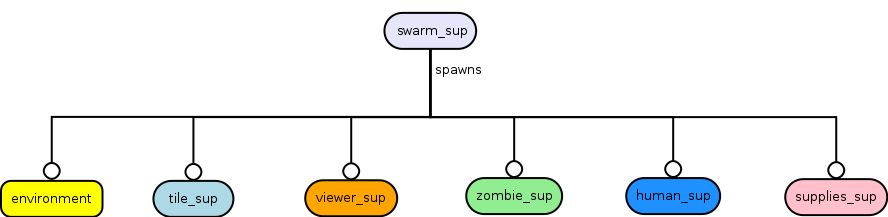
\includegraphics[width=0.4\textwidth]{../img/supervisor.png}
\caption{Supervision Tree for Swarmer}
    \label{fig:sup_tree}
\end{figure}

The system is built a Cowboy HTTP Server

\begin{figure}[h]
  \centering
  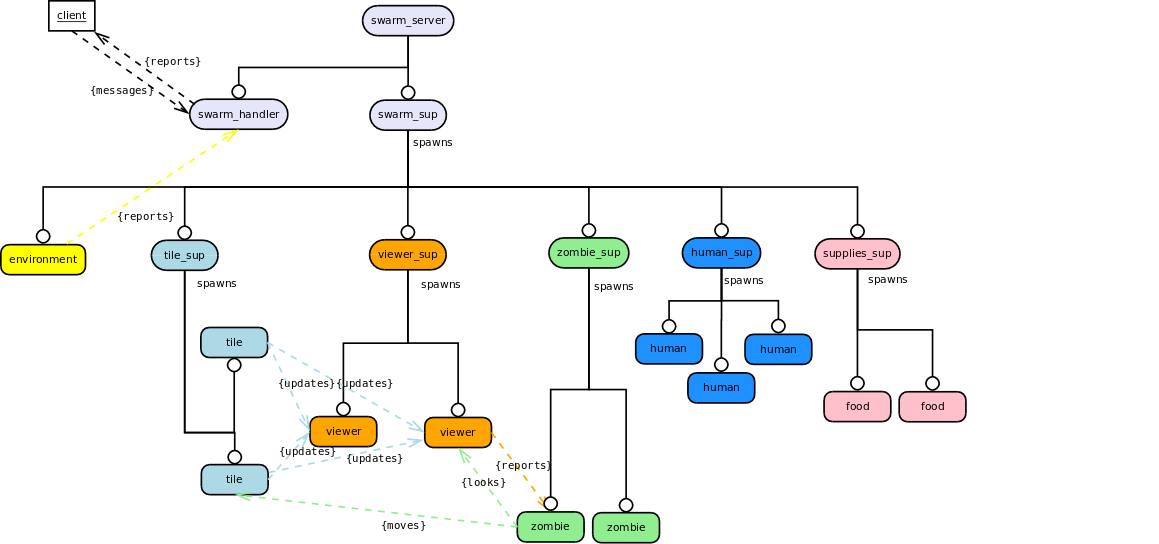
\includegraphics[width=0.4\textwidth]{../img/final_system_ws.png}
\caption{System Architecture}
    \label{fig:system_ws}
\end{figure}

tile/viewery things

% from jake:  how obstructions work in the application
%             system setup

\section{Environment creation \label{environment_creation}}
The creation of an environment begins with the setting of a value for the number of tiles in the grid. As all of our grids are square, there is only a single value for the dimensions of the array. The size of the tile array is determined from the size of the obstruction map selected (section: \ref{obstructions}). Once the dimensionality has been obtained, the grid is constructed through a recursive call to \verb+environment:make_row+ to create an full set of tile processes and corresponding viewer processes. Every tile process is assigned a unique dynamically generated name, which can be used to identify the column and row the tile is positioned in. Tiles can then be identified by using a pair of co-ordinates to derive a tile id. The ability to derive the appropriate tile id through a function call containing co-ordinates is one of the keys to our systems flexibility and the ease of adding new features.\footnote{Tile names are Erlang atoms registered in the supervision tree of the form tileX0Y0}The next stage involves creating a list for each tile of all it's neighbouring viewers. Finally obstructions and entitites are added to each completed tile's state. The system will now be in a paused state, ready to run the simulation.\\
\\
\section{Obstructions \label{obstructions}}
Although we had always planned to include obstructions within our environment, the functionality was a late addition to the simulation. We were concerned with how the resolution would effect our planned inclusion of heuristic path planning.\footnote{Heuristic path planning was one of our unrealised stretch goals.} We decided to implement obstructions at a fraction of the resolution of our natural simulation resolution. As we had previously fixed the size of environment tiles at \(50^2\) we selected a size of \(5^2\) for each of cell of the 'obstruction grid'. Stored in the tile state are obstructed co-ordinates on the obstruction grid scale so in a grid 5 tiles by tiles in size, there are obstruction 'cells' in the range of \( (0,0) \) to \( (49,49) \). One of the primary considerations was to be able draw the environment using a paint tool. We selected mtPaint \footnote{http://mtpaint.sourceforge.net/} due to the ease of exporting images as ascii files.\\
\\
For a standard 5 tile environment we create a plain white image \(50^2\) pixels in size and draw in the required obstructions.

\begin{figure}[h]
  \centering
  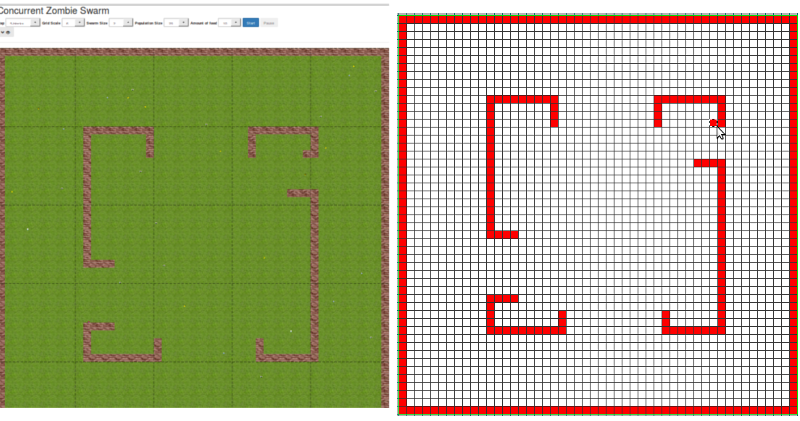
\includegraphics[width=0.4\textwidth]{../img/mt_paint.png}
\caption{Mt Paint}
    \label{fig:mtpaint}
\end{figure}

The resulting ascii file, stripped of line breaks, produces a string of 2500 characters. The string is then processed into an array of indices corresponding to characters representing obstructions. In order to convert an index back into a co-ordinate pair (on the obstruction grid scale) where \(I\) is the index obtained using \[X = I mod 10 and Y = I / 10\].
Once the co-ordinates have been obtained the corresponding tile id can be identified using \(X / 10\) and \(Y / 10\). Each tile contains the subset of obstructions which corresponds to its own geometry. Whenever an entity wishes to perform an operation over the obstruction grid scale, the co-ordinates are simply divided by 5 and compared against the tiles record. This system provides a flexible resolution independant method of modelling obstructions. Although we haven't parameterised the scale of the obstruction grid, it would be trivial to add this functionality.\\
\\
\section{Behaviours and Intelligence \label{behaviours}}
% from rob: boids
%           what are they?
%           different entities and their Intelligence

\section{Client \label{client}}
% from jake: client stuff


% An example of a floating figure using the graphicx package.
% Note that \label must occur AFTER (or within) \caption.
% For figures, \caption should occur after the \includegraphics.
% Note that IEEEtran v1.7 and later has special internal code that
% is designed to preserve the operation of \label within \caption
% even when the captionsoff option is in effect. However, because
% of issues like this, it may be the safest practice to put all your
% \label just after \caption rather than within \caption{}.
%
% Reminder: the "draftcls" or "draftclsnofoot", not "draft", class
% option should be used if it is desired that the figures are to be
% displayed while in draft mode.
%
%\begin{figure}[!t]
%\centering
%\includegraphics[width=2.5in]{myfigure}
% where an .eps filename suffix will be assumed under latex,
% and a .pdf suffix will be assumed for pdflatex; or what has been declared
% via \DeclareGraphicsExtensions.
%\caption{Simulation results for the network.}
%\label{fig_sim}
%\end{figure}

% Note that IEEE typically puts floats only at the top, even when this
% results in a large percentage of a column being occupied by floats.


% An example of a double column floating figure using two subfigures.
% (The subfig.sty package must be loaded for this to work.)
% The subfigure \label commands are set within each subfloat command,
% and the \label for the overall figure must come after \caption.
% \hfil is used as a separator to get equal spacing.
% Watch out that the combined width of all the subfigures on a
% line do not exceed the text width or a line break will occur.
%
%\begin{figure*}[!t]
%\centering
%\subfloat[Case I]{\includegraphics[width=2.5in]{box}%
%\label{fig_first_case}}
%\hfil
%\subfloat[Case II]{\includegraphics[width=2.5in]{box}%
%\label{fig_second_case}}
%\caption{Simulation results for the network.}
%\label{fig_sim}
%\end{figure*}
%
% Note that often IEEE papers with subfigures do not employ subfigure
% captions (using the optional argument to \subfloat[]), but instead will
% reference/describe all of them (a), (b), etc., within the main caption.
% Be aware that for subfig.sty to generate the (a), (b), etc., subfigure
% labels, the optional argument to \subfloat must be present. If a
% subcaption is not desired, just leave its contents blank,
% e.g., \subfloat[].


% An example of a floating table. Note that, for IEEE style tables, the
% \caption command should come BEFORE the table and, given that table
% captions serve much like titles, are usually capitalized except for words
% such as a, an, and, as, at, but, by, for, in, nor, of, on, or, the, to
% and up, which are usually not capitalized unless they are the first or
% last word of the caption. Table text will default to \footnotesize as
% IEEE normally uses this smaller font for tables.
% The \label must come after \caption as always.
%
%\begin{table}[!t]
%% increase table row spacing, adjust to taste
%\renewcommand{\arraystretch}{1.3}
% if using array.sty, it might be a good idea to tweak the value of
% \extrarowheight as needed to properly center the text within the cells
%\caption{An Example of a Table}
%\label{table_example}
%\centering
%% Some packages, such as MDW tools, offer better commands for making tables
%% than the plain LaTeX2e tabular which is used here.
%\begin{tabular}{|c||c|}
%\hline
%One & Two\\
%\hline
%Three & Four\\
%\hline
%\end{tabular}
%\end{table}


% Note that the IEEE does not put floats in the very first column
% - or typically anywhere on the first page for that matter. Also,
% in-text middle ("here") positioning is typically not used, but it
% is allowed and encouraged for Computer Society conferences (but
% not Computer Society journals). Most IEEE journals/conferences use
% top floats exclusively.
% Note that, LaTeX2e, unlike IEEE journals/conferences, places
% footnotes above bottom floats. This can be corrected via the
% \fnbelowfloat command of the stfloats package.




\section{Conclusion}
The conclusion goes here.

% references section

% can use a bibliography generated by BibTeX as a .bbl file
% BibTeX documentation can be easily obtained at:
% http://www.ctan.org/tex-archive/biblio/bibtex/contrib/doc/
% The IEEEtran BibTeX style support page is at:
% http://www.michaelshell.org/tex/ieeetran/bibtex/
%\bibliographystyle{IEEEtran}
% argument is your BibTeX string definitions and bibliography database(s)
%\bibliography{IEEEabrv,../bib/paper}
%
% <OR> manually copy in the resultant .bbl file
% set second argument of \begin to the number of references
% (used to reserve space for the reference number labels box)
\begin{thebibliography}{1}

% \bibitem{IEEEhowto:kopka}
% H.~Kopka and P.~W. Daly, \emph{A Guide to \LaTeX}, 3rd~ed.\hskip 1em plus
%   0.5em minus 0.4em\relax Harlow, England: Addison-Wesley, 1999.

  \bibitem{erlang}
    Ericsson AB,
    \emph{About Erlang},
    \url{http://www.erlang.org/about.html}

  \bibitem{d3}
    Mike Bostock,
    \emph{D3 Website},
    \url{http://d3js.org/}

  \bibitem{occam_boids}
    Fred Barns,
    \emph{GPU Boids},
    \url{http://frmb.org/occam.html#gpuboids}

  \bibitem{erlang_boids}
    Jim Menard,
    \emph{Erlang Boids Simulation Design},
    \url{http://jimmenard.blogspot.co.uk/2007/06/erlang-boids-simulation-design.html}

  \bibitem{boids}
    Craig Reynolds,
    \emph{Boids - Background and Update},
    \url{http://www.red3d.com/cwr/boids/}

  \bibitem{otp}
    Ericsson AB,
	\emph{Open Telecom Platform Design Principles},
    \url{http://www.erlang.org/doc/design_principles/sup_princ.html}

  \bibitem{supervisors}
    Ericsson AB,
	\emph{Erlang Supervisors},
    \url{http://www.erlang.org/doc/man/supervisor.html}

\end{thebibliography}

% that's all folks
\end{document}
